\subsection{Geometric Fiducial Cuts}\label{sec:analysis.fid_cuts}

 A fiducial cut is required to prevent a significant systematic error contribution from either gaining or loosing events that lie in nonuniform regions, such as space between sectors. This cut, shown in Figs.~\ref{fig:pos:fidcut_all},~\ref{fig:neg:fidcut_all}, was applied to all data, real and simulated, presented in the final result shown in Sec.~\ref{sec:results}. The geometric fiducial cuts analysis was performed by Jason Bono of the FIU group. The package for performing these fiducial cuts has three options for the parameters involved in the removal process. These options are ``loose", ``nominal" and ``tight" and refer to the amount of area that is to be cut in the space between the drift chambers. A detailed specification of this cut is given in~\cite{clas.g12.note}. This analysis used the nominal option. To understand the systematic error caused in this fiducial, the measurement from the ``tight" option was compared to the measurement at the nominal option. This is discussed in Sec.~\ref{sec:results.systematics}.

\begin{figure}[h!]\begin{center}
\subfloat[Positive Charge Particle Before Geometric Fiducial Cut][]{ %Feynman diagram of \piz two photon decay
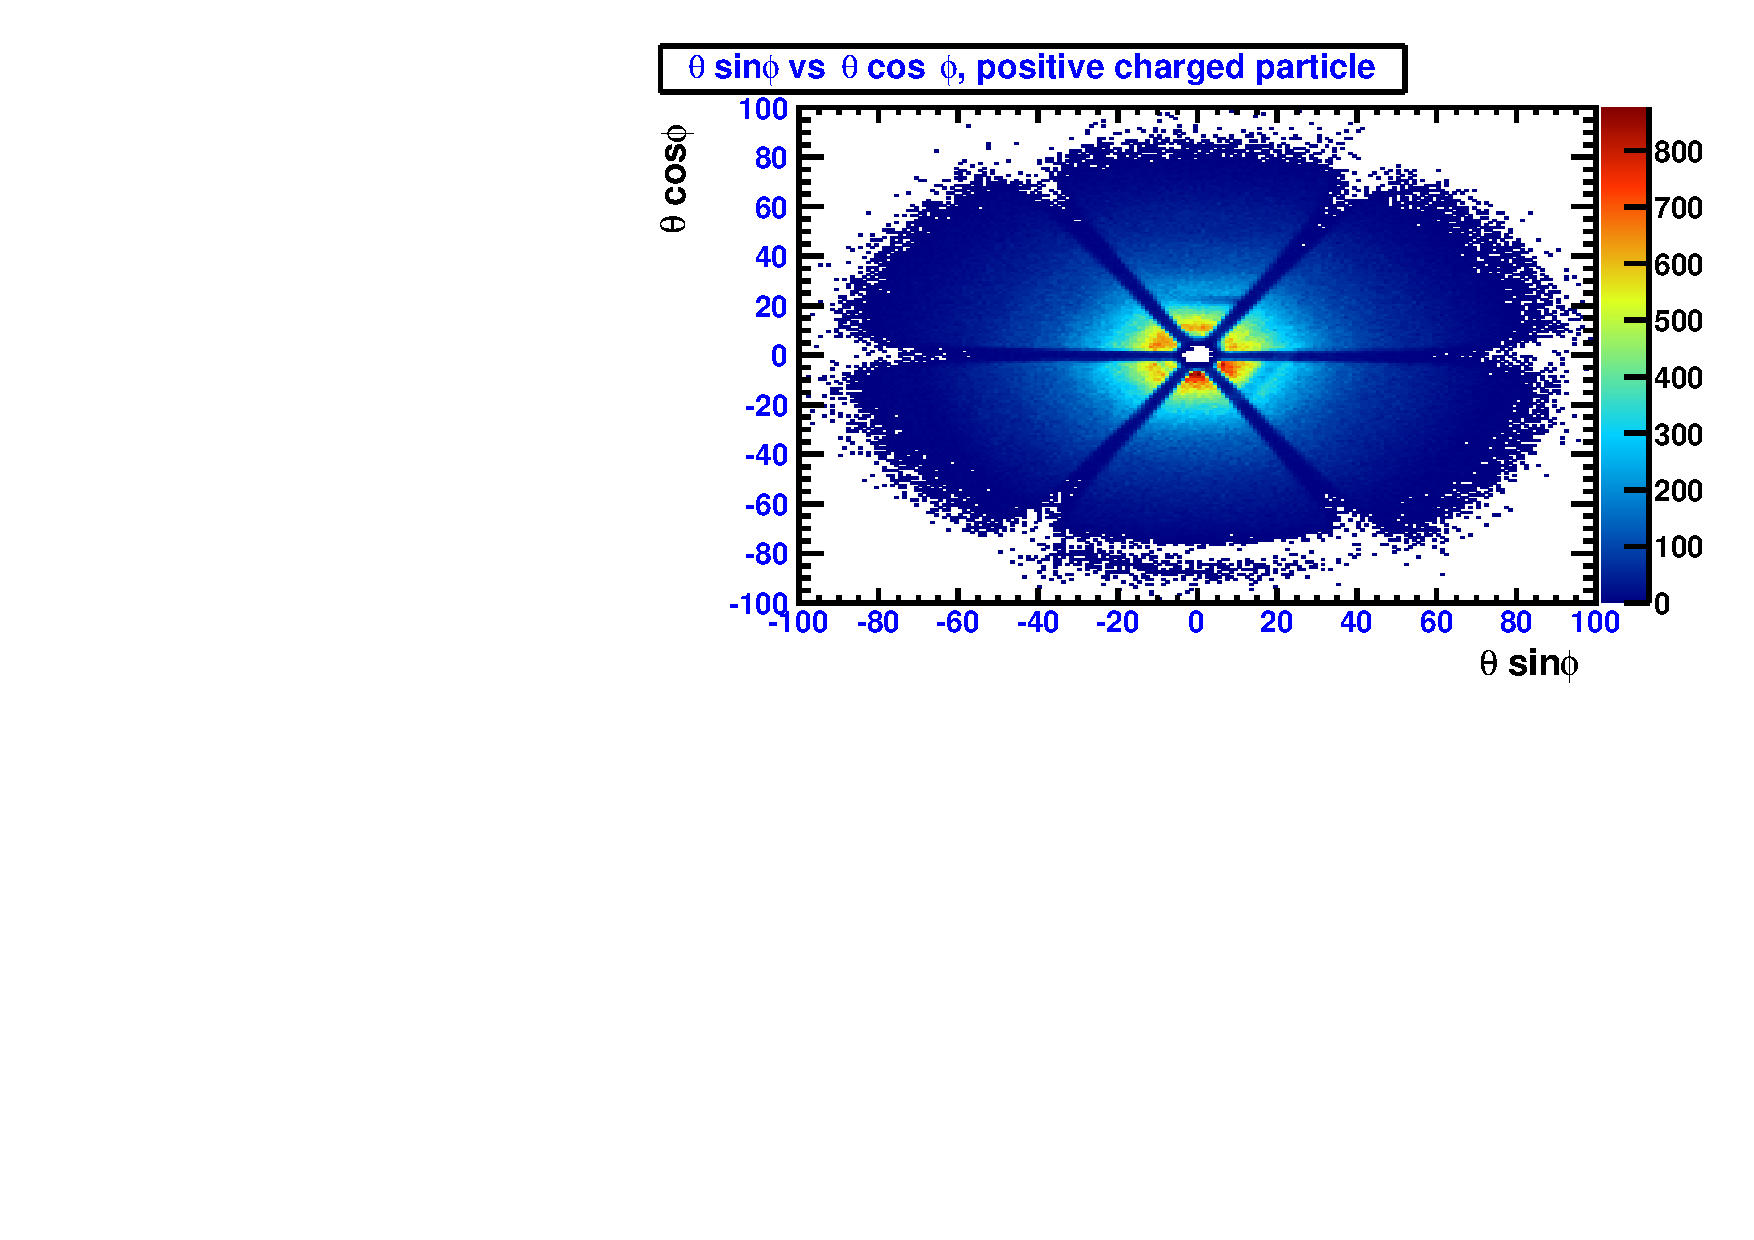
\includegraphics[width=\figwidth,height=\qfigheight]{\grpath/analysis/FIDUCIAL_CUTS/GEOMETRIC/pip_theta_cos_sin_phi_nofid.pdf}\label{fig:pos:fidcut_off}
}\\
\subfloat[Positive Charge Particle After Geometric Fiducial Cut][]{ %Feynman diagram of \piz Dalitz decay
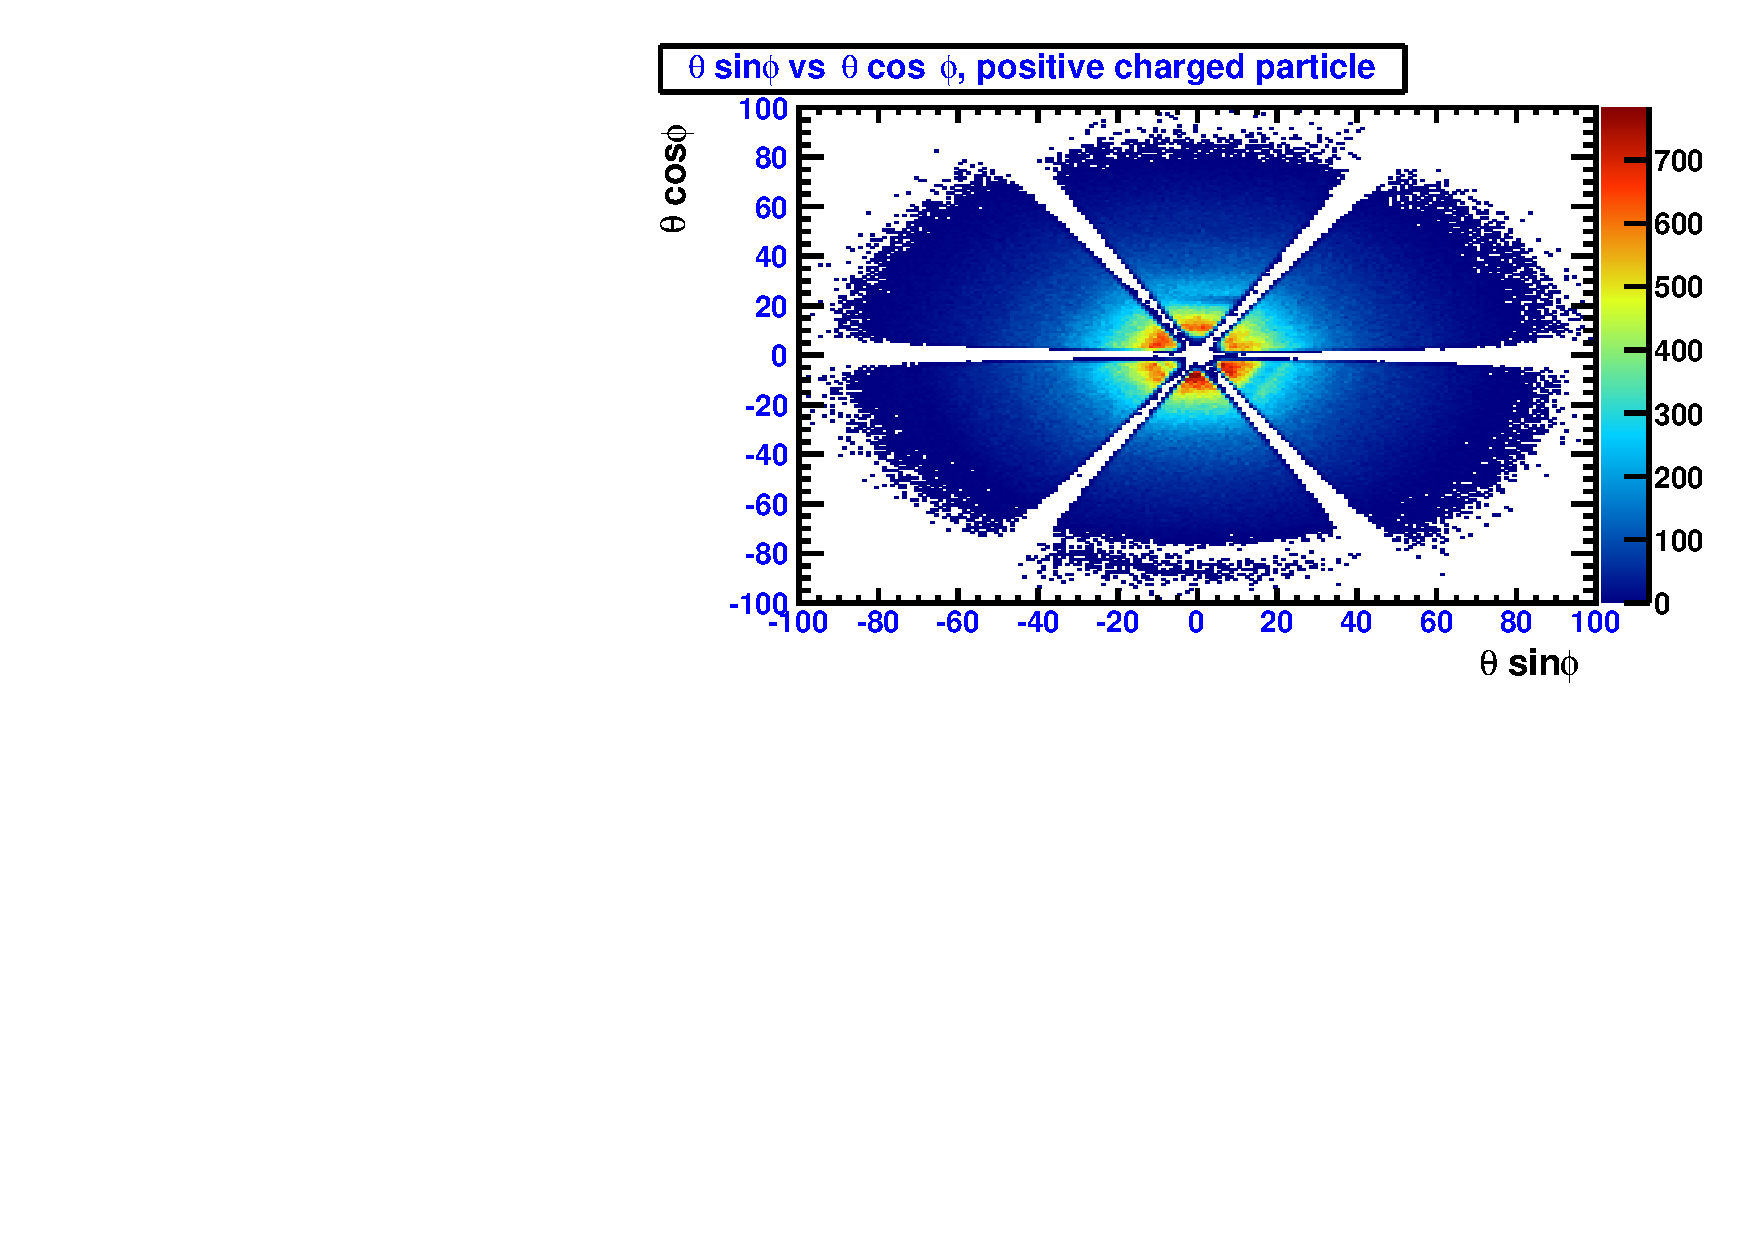
\includegraphics[width=\figwidth,height=\qfigheight]{\grpath/analysis/FIDUCIAL_CUTS/GEOMETRIC/pip_theta_cos_sin_phi_wfid.pdf}\label{fig:pos:fidcut_on}
}
\caption[Positive charged tracks in \abbr{CLAS} \abbr{DC} prior to fiducial cuts being applied, and after being applied]{\label{fig:pos:fidcut_all}Positive charged tracks in \abbr{CLAS} \abbr{DC} prior to fiducial cuts~\subref{fig:pos:fidcut_off} being applied, and after~\subref{fig:pos:fidcut_on} being applied.}

\end{center}\end{figure}
%
\begin{figure}[h!]\begin{center}
\subfloat[Negative Charge Particle Before Geometric Fiducial Cut][]{ %Feynman diagram of \piz two photon decay
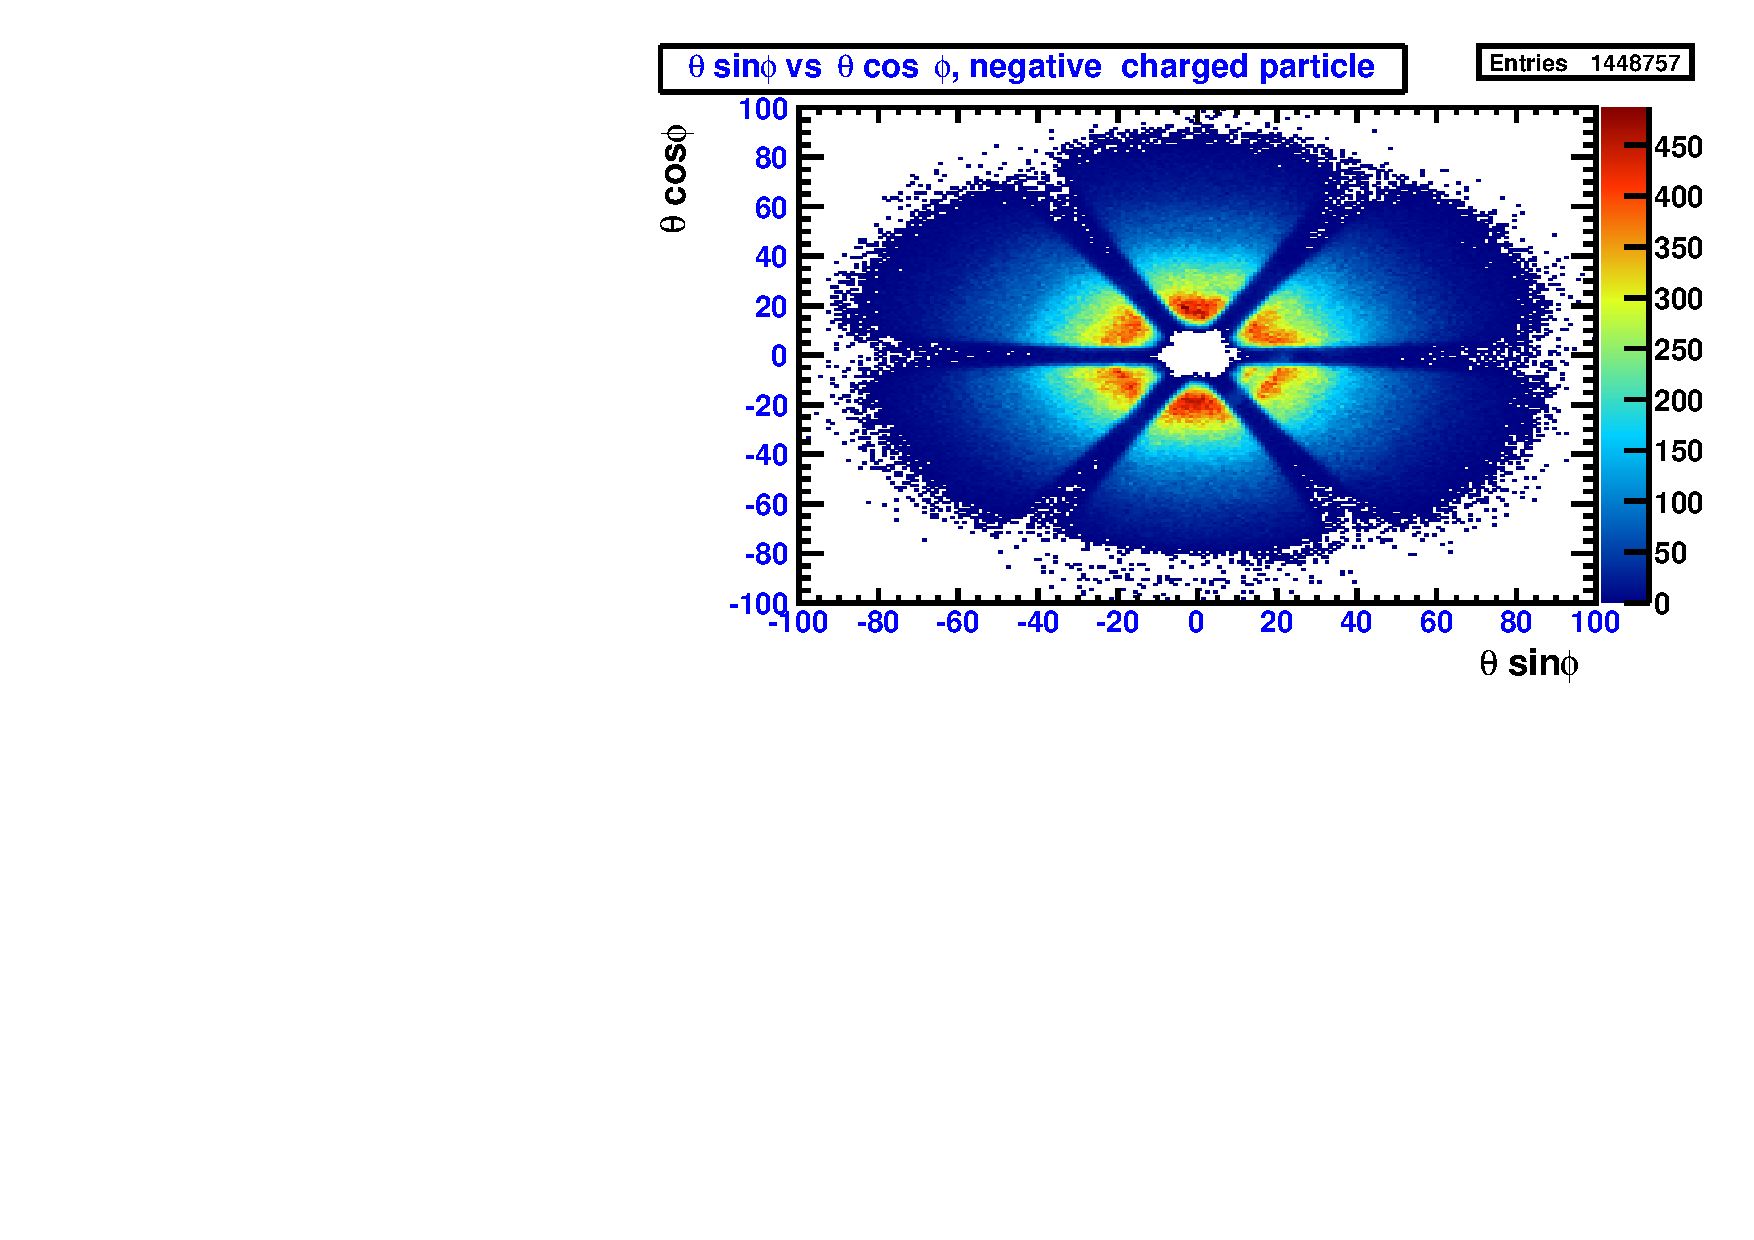
\includegraphics[width=\figwidth,height=\qfigheight]{\grpath/analysis/FIDUCIAL_CUTS/GEOMETRIC/pim_theta_cos_sin_phi_nofid.pdf}\label{fig:neg:fidcut_off}
}\\
\subfloat[Negative Charge Particle After Geometric Fiducial Cut][]{ %Feynman diagram of \piz Dalitz decay
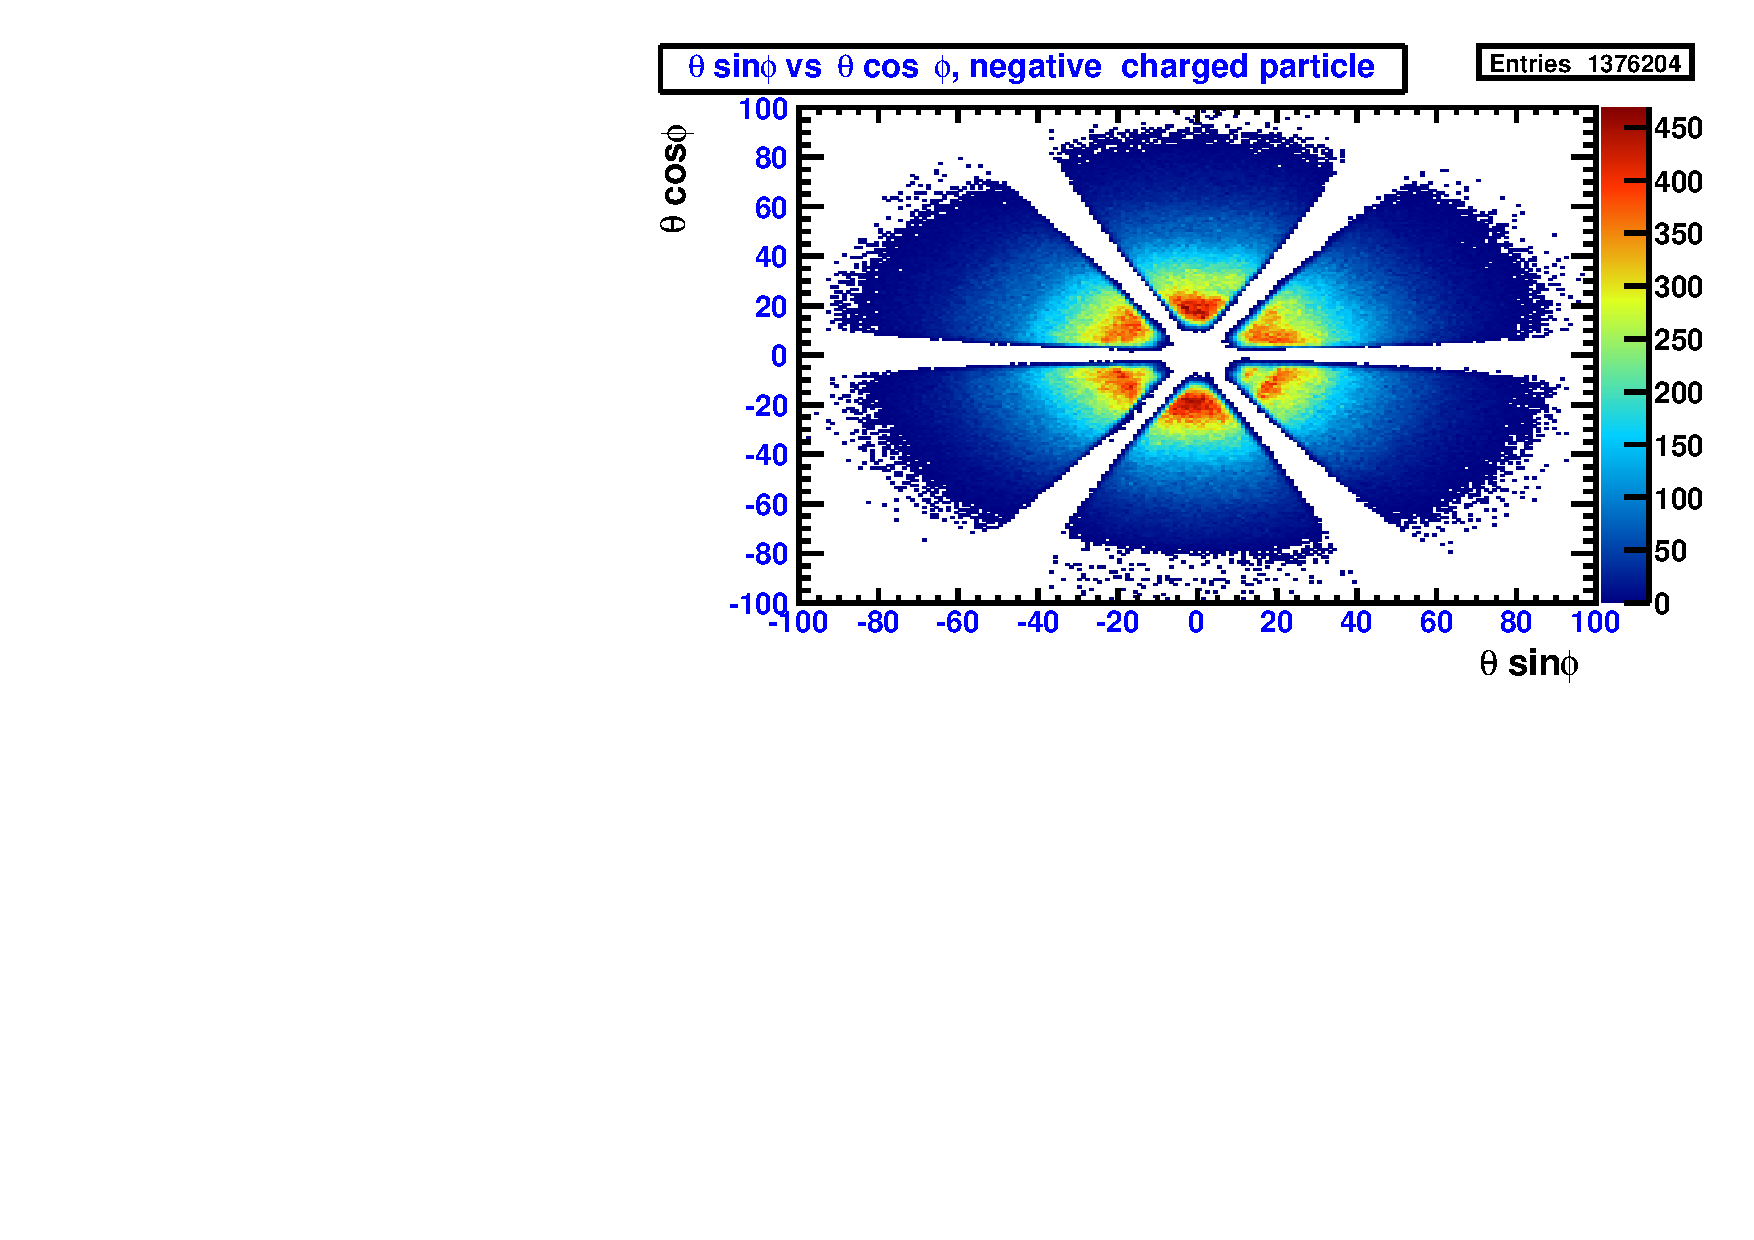
\includegraphics[width=\figwidth,height=\qfigheight]{\grpath/analysis/FIDUCIAL_CUTS/GEOMETRIC/pim_theta_cos_sin_phi_wfid.pdf}\label{fig:neg:fidcut_on}
}
\caption[Negative charged tracks in \abbr{CLAS} \abbr{DC} prior to fiducial cuts being applied, and after being applied]{\label{fig:neg:fidcut_all}Negative charged tracks in \abbr{CLAS} \abbr{DC} prior to fiducial cuts~\subref{fig:pos:fidcut_off} being applied, and after~\subref{fig:pos:fidcut_on} being applied.}

\end{center}\end{figure}

\FloatBarrier
